\documentclass[11pt,a4paper]{extarticle}
\usepackage[margin=1in]{geometry}
\usepackage[utf8]{inputenc}
\usepackage{booktabs} % for toprule, midrule and bottomrule
\usepackage{adjustbox}
\usepackage{amsmath}
\usepackage{bbold}
\usepackage{etoolbox}
\usepackage{setspace} % for \onehalfspacing and \singlespacing macros
\usepackage[hidelinks]{hyperref}
\usepackage{array}
\usepackage{graphicx}
\usepackage{setspace}
\usepackage{caption}
\usepackage{pdflscape}
\usepackage{caption}
\usepackage{tabularx}
\usepackage{authblk}
\usepackage{float}
\usepackage{siunitx}
\usepackage{titlesec}
\usepackage{pgfplots}
\usepackage[authoryear]{natbib}
\usepackage{scrextend}
\usepackage{nicefrac}
\usepackage{enumitem}
\usepackage{multirow}
\usepackage{xcolor}
%\usepackage{showframe}
%\usepackage{lipsum}

% set space
%\doublespacing

% section headings
\renewcommand{\thesection}{\Roman{section}.\hspace{-0.5em}}
\renewcommand\thesubsection{\Alph{subsection}.\hspace{-0.5em}}
\renewcommand\thesubsubsection{\hspace{-1em}}
\newcommand{\subsubsubsection}[1]{\begin{center}{\textit{#1}}\end{center}}

\titleformat{\section}
{\bf\centering\large}{\thesection}{1em}{}

\titleformat{\subsection}
{\itshape\centering}{\thesubsection}{1em}{}

\titleformat{\subsubsection}
{\bf}{\thesubsubsection}{1em}{}

% unicode chars for plots
\DeclareUnicodeCharacter{2212}{$-$}

% booktabs
\setlength\heavyrulewidth{0.06em} % 0.01em> midrule

% images
\graphicspath{ {D:/Users/saketh/Documents/GitHub/BECCS-Case-Study/documents/exhibits/} }

% array
\newcolumntype{L}[1]{>{\raggedright\let\newline\\\arraybackslash\hspace{0pt}}m{#1}}
\newcolumntype{C}[1]{>{\centering\let\newline\\\arraybackslash\hspace{0pt}}m{#1}}
\newcolumntype{R}[1]{>{\raggedleft\let\newline\\\arraybackslash\hspace{0pt}}m{#1}}

% caption set up
\captionsetup[table]{
	font = {sc},
	labelfont = {bf}
}

% sig stars
\def\sym#1{\ifmmode^{#1}\else\(^{#1}\)\fi}

% hyperlinks
\definecolor{darkblue}{RGB}{0,0,150}
\hypersetup{
	colorlinks=true,
	linkcolor = blue,
	urlcolor  = blue,
	citecolor = darkblue,
	anchorcolor = blue
}

% bibliography
\makeatletter
\renewenvironment{thebibliography}[1]
{\section*{References}%
	\@mkboth{\MakeUppercase\refname}{\MakeUppercase\refname}%
	\list{}%
	{\setlength{\labelwidth}{0pt}%
		\setlength{\labelsep}{0pt}%
		\setlength{\leftmargin}{\parindent}%
		\setlength{\itemindent}{-\parindent}%
		\@openbib@code
		\usecounter{enumiv}}%
	\sloppy
	\clubpenalty4000
	\@clubpenalty \clubpenalty
	\widowpenalty4000%
	\sfcode`\.\@m}
{\def\@noitemerr
	{\@latex@warning{Empty `thebibliography' environment}}%
	\endlist}
\makeatother

% etoolbox
\AtBeginEnvironment{quote}{\singlespacing}

% proofs
\newenvironment{proof}[1][Proof]{\noindent\textbf{#1:} }{\ \rule{0.5em}{0.5em}}

\begin{document}

\title{\singlespacing{\textbf{Efficient pollution abatement in electricity markets with intermittent renewable energy}}}

\author[]{Saketh Aleti\thanks{I would like to thank Gal Hochman for helpful comments and the Sun Grant for funding this project. }}

\affil[]{\small{Rutgers University}}

\date{\vspace{-1em}\small{\today}}

\maketitle

\section{Extended Abstract}

Renewable energy technologies have seen considerable adoption over the last few decades (EIA 2019). Unlike the alternatives, wind and solar power are particularly unique in that the amount of energy they supply is intermittent. Consequently, designing economically efficient policy to promote their adoption is not straightforward given that they cannot easily substitute for traditional technologies such as coal power which handles base load demand. Some of the literature has approached the problem by constructing numerical models that find the cheapest renewable technology set while accounting for intermittent supply. Müsgens and Neuhoff (2006) model uncertain renewable output with intertemporal generation constraints, while Neuhoff, Cust, and Keats (2007) model temporal and spatial characteristics of wind output to optimize its deployment in the UK. On the other hand, other literature focuses on the effect of intermittent technologies on the market itself; Ambec and Crampes (2010) study the interaction between intermittent renewables and traditional reliable sources of energy in decentralized markets, and Chao (2011) models alternative pricing mechanisms for intermittent renewable energy sources. Additionally, Borenstein (2010) reviews the effects of present public policies used to promote renewables and the challenges posed by intermittency. 

In this paper, we present a theoretical model of electricity markets with intermittent renewable energy and derive the optimal public policy to handle pollution externalities. In contrast with other theoretical models of intermittency which optimize a pubic electricity sector, our model assumes utility and profit maximization. Additionally, it represents the energy sector over multiple periods with electricity output for each technology varying over time for intermittent technologies. This approach is better suited for studying the dynamics of present US electricity markets which are primarily funded by private sector investment and have prices that vary over time. We first consider a simpler version of our model with two periods and two energy generation technologies, derive the comparative statics for this model, and detail the policy implications. Then, we produce numerical results for optimal policy prescriptions with a multi-period, multi-technology version of our model using electricity generation data on the PGM region.

Present models of the energy sector concerned with the adoption of renewable energy often discuss the elasticity of substitution between clean and dirty energy; this elasticity is meant to capture factors such as intermittency and reliability that impede perfect substitution between energy sources. Additionally, this elasticity is often estimated empirically or modelled in a CGE using a CES production function with capital inputs for each energy technology. However, this top down approach may be missing the actual source of the substitution effects while also being unrealistic. For instance, consider a simple case where energy output is a Cobb-Douglas function (a special case of CES) of two energy inputs: solar and coal. According to this function, increasing the amount of coal input causes the marginal product of solar input to rise; this makes little sense in practical terms, since the output of additional solar panels should not be related to the amount of coal input. Moreover, this approach, while possibly relevant for other sectors' goods, weakens the accuracy of theoretical and CGE models focused on the energy sector.

However, it is still possible to produce a more accurate model of the electricity sector that can capture trade-offs between the energy output of different technologies from both cost and intermittency. To start, rather than energy production following a general CES function, we first assume that energy follows a linear production function where total energy is instead the sum of the energy output of each source. The purpose of using a linear production function is that increasing the input of one energy source does not change the marginal product of another source as it does in a CES function. Additionally, we split this production function up across periods; that is, in each period, the electricity generation is equal to the energy output of each source in that period. For intermittent technologies, energy output varies in each period, so total output would as well. Next, we assume that firms pick a profit-maximizing level of investment in each energy technology. This investment stays fixed in all periods, but the total energy output can vary over time due to intermittency; for instance, a solar plant provides a variable output by time of day, while nuclear plant cannot easily vary its output within 24 hours. Moreover, we assume that firms face linear costs and electricity prices are set equal to their marginal cost; the former assumption is temporarily made for mathematical tractability while the latter is realistic given the competitiveness of electricity markets. 

While the production function described so far is linear, we may still find a non-zero elasticity of substitution between energy sources. That is, consider a representative agent with a CES utility function that captures intertemporal variation in the utility gained from energy consumption. Specifically, the utility function is composed of energy consumption differentiated by period; so, for example, in a two-period model, we may have off-peak consumption and on-peak consumption as our two goods. Because people prefer to consume energy at different proportions based on the time of day, this variation can be modeled through the share parameters in the CES function. Moreover, since people may substitute energy consumption across time by availability and prices, the CES elasticity parameter captures the intertemporal elasticity of substitution. Thus, in this model, the intermittency of an energy generation technology plays a key role in determining its substitutability with other technologies. For instance, solar power may be a good substitute for coal power during the day, but obviously not at night; consequently, this pair complements each other, since coal handles the base load while solar handles the peak load. Alternatively, wind and solar are a poor combination, since both produce intermittently; this pair is closer to being substitutes. All in all, the result of using CES preferences with temporally differentiated energy consumption is that we can capture substitutability/complementarity between energy sources in an accurate way. 

The first significant result in this model is that the optimal quantity of investment in intermittent renewable technology is concave with respect to both cost efficiency (cost per unit) and output efficiency (energy output per unit). So, for example, suppose some location has a coal-fired plant and is considering investing in a solar power plant. A 10\% increase in the output per solar panel may increase the optimal quantity of solar panels by x\%, while a 20\% increase in solar efficiency will increase the optimal quantity of solar by y\% where y < 2x. Because of this concavity, exponential increases in efficiency of intermittent renewable sources over time, as Moore’s Law may predict, is not enough to fully substitute out reliable energy technology. Hence, we argue that a full transition to renewable energy requires more emphasis on technologies such as nuclear, biomass, hydro, and geothermal energy sources; although these sources compete with intermittent energy technology, they are able fully substitute out for fossil fuel energy. Additionally, the reliable output of these technologies can handle base loads; this allows them to complement the intermittency of renewables such as wind and solar. 

Secondly, suppose that we would like to promote clean energy adoption and replace dirty energy to reduce the pollution emissions. Because we have diminishing returns from both forms of efficiency, it is optimal to subsidize both research and the cost of intermittent renewable technology. This is because we expect research subsidies to increase both output efficiency and cost efficiency, while subsidies would increase the cost efficiency of renewables for a market participant. A mix of both instruments leads to improving both forms of efficiency at once, thus replacing dirty energy technology in the most cost-efficient way. Alternatively, since we would see symmetrical effects from taxing dirty energy sources rather than subsidizing clean ones, taxing dirty energy sources can substitute for renewable cost subsidies. Consequently, a carbon tax plus a research subsidy for renewables is another optimal choice for pollution abatement. 

Finally, our model implies that the optimal level of subsidies/taxes on energy generation should vary by the state of the local energy market. That is, the change in optimal quantity of intermittent energy technology with respect to both types of efficiency is also a function of the efficiencies of the other technologies available. Consequently, the marginal benefit of a subsidy or tax varies spatially, since different geographies have access to different energy sources. For instance, one community may be relying on hydropower while another may be using coal power; the effect of a 1\% cost subsidy on solar installments in these two communities would vary because of the differences in the communities’ pre-existing energy generation technologies. Hence, local communities that aim to promote clean energy and reduce pollution should optimize their policy instruments to suit their local energy markets. 


\subsection{References}

\begin{itemize}
	\item Literature
	\item Description of model
	\item 
\end{itemize}



\section{Outline}
\dots

Things I'd like to say:
\begin{itemize}
	\item Because the marginal product of renewable energy inputs may be time-dependent, renewable energy may complement traditional, constant-output energy sources rather than fully substitute for it. Obvious arugment follows from base load output required at all times. 
	\item How the conversion parameters for energy inputs affect their elasticity of substitution
	\item How variability in energy output decreases the value of particular energy sources. Obvious argument from concavity of utility implying risk aversion. 
\end{itemize}

\pagebreak

\section{Introduction}

Renewable energy technologies have seen considerable adoption over the last few decades (EIA 2019). Unlike the alternatives, wind and solar power are particularly unique in that the amount of energy they supply is intermittent. Consequently, designing economically efficient policy to promote their adoption is not straightforward given that they cannot easily substitute for traditional technologies such as coal power which handles base load demand. Moreover, simpler approaches, such as using the levelized cost of electricity (LCOE) to compare technologies is flawed in any setting with variable electricity prices. In particular, \citet{Joskow2011} argues that 

\begin{quote}
	``Instead [of using metrics like LCOE], the economics of all generating technologies, both intermittent and dispatchable, can be evaluated based on the expected market value of the electricity that
	they will supply, their total life-cycle costs, and their associated expected profitability. Such an
	analysis would reflect the actual expected production profiles of dispatchable and intermittent
	technologies, the value of electricity supplied at different times, and other costs of intermittency
	associated with reliable network integration. This is exactly the way investors in merchant generating plants evaluate whether or not to invest."
\end{quote}
We structure our model with this critique in mind. Specifically, we develop a model where producers optimize the supply of each generation technology on the expected market value of the electricity produce. We do so by ....

Some of the literature has approached the problem by constructing numerical models that find the cheapest renewable technology set while accounting for intermittent supply. \citet{MN2006} model uncertain renewable output with intertemporal generation constraints, while \citet{NCK2007} model temporal and spatial characteristics of wind output to optimize its deployment in the UK. On the other hand, other literature focuses on the effect of intermittent technologies on the market itself; \citet{AC2012} study the interaction between intermittent renewables and traditional reliable sources of energy in decentralized markets, and \citet{Chao2011} models alternative pricing mechanisms for intermittent renewable energy sources. Additionally, \citet{Boren2012} reviews the effects of present public policies used to promote renewables and the challenges posed by intermittency. 

Our model comes closest to that of \citet{HH} who build a peak-load pricing model where the availability of renewable capacity varies stochastically. This stochastic variability models the intermittency and affects the adoption of renewables in a market with dynamic pricing. Furthermore, they simplify their analysis by setting aside complications such as  outage costs and rationing rules. In total, their model finds an S-shaped adoption curve for renewables once their LCOE's reach those of fossil fuel energy. In addition, they find that a Pigouvian tax can properly internalize the costs of fossil fuels in a setting with perfect competition. Likewise, our model makes equivalent simplifications and finds similar results on an equilibrium in  amarket with dynamic prices. But, our representation of the intermittency of renewables differs in a significant way. 


To highlight this difference, we must first contrast the terms  \textit{intermittency} and \textit{reliability}. By intermittency, we predictable changes in output related to physical constraints. For instance, while wind energy output varies over time, if  we know the angle and speed of wind, we may precisely derive the quantity of energy that a wind farm generates.\footnote{\citet{Foley2012} provide a review of the literature on the forecasting of wind power. Over time, forecasts have gotten much more accurate allowing electricity grids to manage wind power intermittency ahead of time.}  At the same time, these forecasts may not be perfect and, as a result, we see unexpected variation in the output of a technology. This unpredictability may be better captured by the notion of reliability; specifically,  we refer to definition provided by the US Department of Energy's \citep{ORNL} -- ``Power reliability can be defined as the degree to which the performance of the elements in a bulk system results in electricity being delivered to customers within accepted standards and in the amount desired." This is more so related to the stochastic or unpredictable variation in the output of a technology. Unlike intermittency, this cannot be planned around with 100\% certainty. A practical example may be a wind turbine's systems failing. While we may know the chances of this occurring, it's not possible to know when it will occur ahead of time; consequently, this may result in a temporary reduction in the quantity and quality of the electricity delivered --  a loss of reliability. In short, when \citeauthor{HH} define renewable output as equal to a baseline capacity multiplied by a uniform random variable, their model is closer to one of reliability rather than intermittency. 

On the other hand, we neglect reliability for parsimony and develop a two-technology, two-period model consisting of fossil and renewable energy. Then, we model intermittency as defined above by allowing the output of renewable energy to differ between periods according to known function. At the same time, we consider a representative consumer whose utility is given by CES function where each good is electricity consumption differentiated by time. This captures consumers' preferences for electricity consumption throughout the day as well as their willingness to substitute consumption across time. We then fit the parameters of this CES utility function using electricity consumption and price data for each US state. At the same time, we set parameters of our technologies (their cost and output) to those of coal and solar. Overall, this treatment of intermittency produces some key results similar to that of Helm and Mier. That is, we also find a Pigovian tax to be a solution to externalities along with an S-shaped adoption curve for renewables. But, moreover, we find the elasticity of substitution between fossils and renewables to be highly non-linear; this directly challenges the CES production structure assumption made by standard models of fossil and renewable energy. Finally, we discuss how a combination of carbon taxes and research subsidies may be more optimal than carbon taxes alone in the presence of intermittency. 


% What we have in common
% What's new, what adds to the literature


%%%%%%%%%%%%%%%%%%%%%%%%%%%%%%%%%
%%%%%%%% Summary of results
%%%%%%%%%%%%%%%%%%%%%%%%%%%%%%%%%

\section{Model}

We model electricity as a heterogenous good which is differentiated by its delivery time. Then, we consider a representative consumer who purchases varying quantities of electricity in each period in order to maximize utility. Generally, people prefer to spread their electricity consumption out over time; the convexity of the indifference surfaces of a standard CES function can model this preference in a simple way. The use of a CES function for modeling consumer utility with electricity consumption differentiated by time has been explored earlier by \citet{Moha2016}. Their paper calibrates the share parameters of the CES function with actual electricity consumption data for peak and off-peak hours; they further provide a sensitivity analysis with respect to the elasticity of substitution parameter. Similarly, \citet{Schwarz} provides an empirical study of this CES function and estimate its parameters for industrial customers in a real-time pricing program; their estimates of the intertemporal elasticity of substitution for electricity consumption fall around 0.03. 

Next, we model the electricity sector using a representative firm that chooses a set of electricity-generating inputs to maximize profit; some of these inputs are intermittent - they generate a differing amounts of energy in each period. These two sides of the market reach an equilibrium through adjustments in prices of electricity in each period.\footnote{While, in reality, consumers generally pay fixed rates for electricity, \citeauthor{HH} provide a motivation for models incorporating dynamic pricing; they argue such approaches to pricing will become the norm with further technological advances and coming regulatory changes. } For simplicity, we do not allow for load rationing  or negative prices. And, again for simplicity, we assume that the output of all technologies in each period does not vary stochastically. 

\subsection{General Model}

Consumers purchase variable amounts of electricity $Z_t$ over each period $t$. Additionally, assuming that the price of electricity in each period is held constant, they prefer to ration their electricity usage across each period in fixed proportions. And, lastly, we presume that consumers would be willing to shift their consumption from one period to another in response to a shift in prices. Overall, these assumptions can be captured using a a standard CES utility function
\begin{equation}
U = \left( \sum_t \alpha_t Z_t^\phi  \right)^{1/\phi}
\end{equation}
where $\sigma = 1/(1-\phi)$ is the intertemporal elasticity of substitution for electricity consumption. We define $\sum_t \alpha_t = 1$, so that $\alpha_t$ is the fraction of electricity consumption in period $t$ when all prices are equal; naturally, $\alpha_t > 0$ for all $t$. We assume that any discounting over time is absorbed into $\alpha$ for parsimony.The budget constraint is given by
\begin{equation}
I = \sum_t p_t Z_t
\end{equation}
where $p_t$ is the price of electricity in period $t$ and $I$ is the income. Furthermore, since CES preferences are homothetic, we may aggregate the consumers into a single representative consumer. Consequently, the first order conditions four our representative consumer when maximizing utility given this budget constraint imply:
\begin{align}
Z_t &= \left(\frac{\alpha_t}{p_t} \right)^\sigma \frac{I}{P} \\
P &= \sum_t \alpha_t^\sigma p_t^{1-\sigma}
\end{align}
where $P$ is the price index. Note that this model naturally does not allow for blackouts in equilibrium, since the price of electricity in any period gets arbitrarily large as the quantity of energy consumed in that period approaches 0. Furthermore, note that prices must be positive; although this is sometimes violated in reality, we do not believe that this assumption significantly affects our analysis. 

Secondly, we have firms maximizing profit by picking an optimal set of energy inputs. In reality, electricity markets are fairly competitive, so we can model the set of firms by using a single representative firm that sets marginal revenue equal to marginal cost. We define the quantity of deployed energy technology $i$ as $X_i$, and we define its output per unit in period $t$ as $\xi_{1,t}$. So, for example, if $i$ is solar power, $X_i$ would be the number of solar panels and $\xi_{i,t}$ may be kW generated per solar panel in period $t$. Consequently, the energy generated in period $t$, $Z_t$, is given by $\sum_i \xi_{i,t} X_i$. We define these variables in matrices to simplify notation:
\begin{align*}
X \equiv \begin{pmatrix}
X_1\\
\vdots\\
X_n
\end{pmatrix} ,\;
Z \equiv \begin{pmatrix}
Z_1\\
\vdots\\
Z_m
\end{pmatrix} ,\;
p \equiv \begin{pmatrix}
p_1\\
\vdots\\
p_m
\end{pmatrix} ,\;
\xi \equiv \begin{pmatrix}
\xi_{1,1} & \dots & \xi_{1,m}\\
\vdots & \ddots & \\
\xi_{n,1} &  & \xi_{n,m}
\end{pmatrix} 
\end{align*}
where we have $n$ technologies, $m$ periods, and $Z \equiv \xi^T X$. A key element of this model is that $X$ does not vary by time. This is important, because the time scale of our model must be fairly granular to study the effects of intermittency. So, for instance, we may have $t \in \{ 1, \dots, 24\}$ representing each hour of the day. In such short time scales, we can safely assume that producers do not modify the quantity of the technology they employ. Moreover, this keeps the model parsimonious by preventing more complicated dynamics from entering the producers optimization problem. 

Instead, our representative firm sets $X$ once to maximize profit in all periods while facing the cost function $C(X_1, \dots, X_n)$.  \citet{HH} note that past literature has argued for concave cost functions in the energy market due to effects such as economics of scale and learning by doing; on the other hand, standard cost functions are generally convex. So, like Helm and Meir, we take an intermediate approach by using a linear cost function. Specifically, we have $C(X) \equiv \sum_i c_i X_i \equiv c^T X$ where $c_i$ is the cost per unit of $X_i$. Total profit is given by 
\begin{equation}
\Pi = p^T Z - c^T X
\end{equation}
To simplify the algebra, we set the number of technologies equal to the number of periods $(n=m)$. Additionally, we further require that the output per unit of each technology is unique and non-negative in each period; in other words, the output per unit of one technology is not a linear combination of those of the other technologies in our set. This then implies that $\xi$ is of full rank and therefore invertible.  Now, maximizing profit, we find the first order condition:
\begin{equation}
\frac{\partial \Pi}{\partial X} = 0 \implies p = \xi^{-1} c
\end{equation}
Combining both first order conditions allows us to find the equilibrium. The equilibrium results any number of technologies ($n$) are analytic, but they are difficult to interpret due to the number of parameters involved. Hence, in order to produce more comprehensible results, we proceed with a special case of our general model. 

\subsection{Cobb-Douglas Case with Two Periods \& Two Technologies}

\subsubsection{Equilibrium Results}

Firstly, we restrict the utility function to its Cobb-Douglas form which is simply the case where the elasticity of substitution $\sigma = 1$. Secondly, we limit the number of periods and technologies to 2. And, thirdly, we normalize the prices such that the budget $I$ is $1$. Consequently, our demand equations simplify to:
\begin{align}
Z_t &= \alpha_t / p_t \\
Z_s &= \alpha_s / p_s
\end{align}
where $t$ and $s$ are our two periods. Next, solving for the FOC condition for profit maximization, we have:
\begin{align*}
p &=  \xi^{-1} c \\
p &= \begin{pmatrix}
-\dfrac{c_{1}\,\xi _{\mathrm{2s}}-c_{2}\,\xi _{\mathrm{1s}}}{\xi _{\mathrm{1s}}\,\xi _{\mathrm{2t}}-\xi _{\mathrm{1t}}\,\xi _{\mathrm{2s}}}  \\[2ex]
\dfrac{c_{1}\,\xi _{\mathrm{2t}}-c_{2}\,\xi _{\mathrm{1t}}}{\xi _{\mathrm{1s}}\,\xi _{\mathrm{2t}}-\xi _{\mathrm{1t}}\,\xi _{\mathrm{2s}}} 
\end{pmatrix} 
\end{align*}
And, substituting back into our demand equations, we find the equilibrium quantities for $Z$ and $X$. 
$$
Z = \begin{pmatrix}
\dfrac{\alpha _{t}\,\left(\xi _{\mathrm{1s}}\,\xi _{\mathrm{2t}}-\xi _{\mathrm{1t}}\,\xi _{\mathrm{2s}}\right)}{c_{2}\,\xi _{\mathrm{1s}} - c_{1}\,\xi _{\mathrm{2s}}} \\[2ex]
\dfrac{\alpha _{s}\,\left(\xi _{\mathrm{1s}}\,\xi _{\mathrm{2t}}-\xi _{\mathrm{1t}}\,\xi _{\mathrm{2s}}\right)}{c_{1}\,\xi _{\mathrm{2t}}-c_{2}\,\xi _{\mathrm{1t}}} 
\end{pmatrix}
\implies 
X = \begin{pmatrix}
\dfrac{\alpha _{t}\,\xi _{\mathrm{2s}}}{c_{1}\,\xi _{\mathrm{2s}}-c_{2}\,\xi _{\mathrm{1s}}}+\dfrac{\alpha _{s}\,\xi _{\mathrm{2t}}}{c_{1}\,\xi _{\mathrm{2t}}-c_{2}\,\xi _{\mathrm{1t}}} \\[2ex] 
-\dfrac{\alpha _{t}\,\xi _{\mathrm{1s}}}{c_{1}\,\xi _{\mathrm{2s}}-c_{2}\,\xi _{\mathrm{1s}}}-\dfrac{\alpha _{s}\,\xi _{\mathrm{1t}}}{c_{1}\,\xi _{\mathrm{2t}}-c_{2}\,\xi _{\mathrm{1t}}}
\end{pmatrix}
$$

Furthermore, we derive restrictions on the parameters $\xi$ and $c$ by assuming $Z, X > 0$. These restrictions are detailed in \hyperref[tab:paramrest]{Table 1}. There are two possible sets of symmetrical restrictions. The first set, Case 1, assumes that technology 2 is more cost effective in period $t$, while the second set, Case 2, assumes that technology 1 is more cost effective in period $t$. If a given set of parameters do not fall into either case, we are left with an edge case where one of the technologies is not used. Additionally, these inequalities compare two types of efficiency -- output efficiency and cost efficiency; we define output efficiency as electricity output per unit of input and cost efficiency in terms of electricity output per dollar of input. We refer to the last set of restrictions as mixed, because they relate both cost and output efficiency. 


\begin{table}[h!]
	\caption{Parameter Restrictions for $Z, X > 0$} 
	\label{tab:paramrest}
	\small
	\centering
	\begin{tabular}{@{\extracolsep{2em}}l@{\hspace{-0.5 em}}cc}
		\\[-4ex]
		\toprule \\[-2.5ex]
		& \textbf{Case 1} & \textbf{Case 2 } \\
		\cmidrule(lr){2-2} \cmidrule(lr){3-3} \\[-1.5ex]
		\textbf{Cost Efficiency}& $\xi_{2t}/c_2 > \xi_{1t}/c_1$ & $\xi_{2t}/c_2 < \xi_{1t}/c_1 $\\
		\textbf{Restrictions} & $\xi_{1s}/c_1 > \xi_{2s}/c_2$  & $\xi_{1s}/c_1 < \xi_{2s}/c_2 $ 		\\ [3ex]
		\textbf{Output Efficiency}& $\xi_{2t}/\xi_{2s} > \xi_{1t}/\xi_{1s}$ & $\xi_{2t}/\xi_{2s} < \xi_{1t}/\xi_{1s}$\\
		\textbf{Restrictions} & $\xi_{1s}/\xi_{1t} > \xi_{2s}/\xi_{2t} $  & $\xi_{1s}/\xi_{1t} < \xi_{2s}/\xi_{2t}  $ 		\\ [3ex]
		\multirow{2}{10em}{\textbf{Mixed Efficiency Restrictions}}& $\dfrac{\alpha_s \left(\xi_{1s}/c_1 - \xi_{2s}/c_2\right)}{\alpha_t \left( \xi_{2t}/c_2 - \xi_{1t}/c_1 \right)} > \xi_{2s}/\xi_{2t}$ & $\dfrac{\alpha_s \left(\xi_{1s}/c_1 - \xi_{2s}/c_2\right)}{\alpha_t \left( \xi_{2t}/c_2 - \xi_{1t}/c_1 \right)} < \xi_{2s}/\xi_{2t}$\\
		& $\dfrac{\alpha_s \left(\xi_{1s}/c_1 - \xi_{2s}/c_2\right)}{\alpha_t \left( \xi_{2t}/c_2 - \xi_{1t}/c_1 \right)} < \xi_{1s}/\xi_{1t} $  & $\dfrac{\alpha_s \left(\xi_{1s}/c_1 - \xi_{2s}/c_2\right)}{\alpha_t \left( \xi_{2t}/c_2 - \xi_{1t}/c_1 \right)} > \xi_{1s}/\xi_{1t} $ 		\\[2ex] 
		\midrule
		\multicolumn{3}{@{}p{40em}@{}}{\footnotesize \textit{Note: } The inequalities in this table assume that all elements of $\xi$ are greater than $0$. The full proof given below provides equivalent restrictions for the zero cases.   }  
	\end{tabular} 
\end{table}

\hfill\\
\begin{proof}
	We aim to derive conditions on $\xi$ and $c$ required to have positive $Z$ and $X$, so we begin by assuming $X, Z  > 0$. Second, since the equations so far are symmetrical, note that there be two symmetrical sets of potential restrictions we must impose on the parameters. Thus, we first assume the inequality $c_1 \xi_{2t} - c_2 \xi_{1t} > 0$ to restrict ourselves to one of the two cases. This assumption results in the denominator of $Z_s$ being positive. Hence, we must also have $\xi_{1s}\xi_{2t} - \xi_{2s}\xi_{1t} > 0 $ for $Z_s > 0$. This same term appears in the numerator for $Z_t$, hence its denominator must be positive: $c_2 \xi_{1s} - c_1 \xi_{2s} > 0$. Now, rewriting these inequalities, we have:
	\begin{align*}
	c_1 \xi_{2t} - c_2 \xi_{1t} > 0 &\implies \xi_{2t}/c_2 > \xi_{1t}/c_1 \\
	c_2 \xi_{1s} - c_1 \xi_{2s} > 0 &\implies \xi_{1s}/c_1 > \xi_{2s}/c_2 \\
	\xi_{1s}\xi_{2t} - \xi_{2s}\xi_{1t} > 0 &\implies \xi_{1s}/\xi_{1t} > \xi_{2s}/\xi_{2t} \\
	&\implies \xi_{1t}/\xi_{1s} < \xi_{2t}/\xi_{2s} 
	\end{align*}
	Note that the latter two restrictions can be derived from the former two. Additionally, we implicitly assume that we have $\xi > 0$. However, this is not necessary assumption, since $\xi$ invertible only requires $\xi_{1t} \xi_{2s} > 0$ or $\xi_{1s} \xi_{2t} > 0$. Instead, we may leave the latter two inequalities in the form $ \xi_{1s}\xi_{2t} > \xi_{2s}\xi_{1t}$ which remains valid when values of $\xi$ are equal to $0$. Lastly, the mixed efficiency restrictions come from $X > 0$. To start, for $X_1$, we have:
	\begin{align*}
	X_1 > 0 &\implies (\alpha_t \xi_{2s})(c_1 \xi_2t - c_2\xi_1t) + (\alpha_s \xi_{2t})(c_1 \xi_{2s} - c_2 \xi_{1s}) < 0\\
	&\implies (\alpha_t \xi_{2s})(c_1 \xi_2t - c_2\xi_1t) < (\alpha_s \xi_{2t})(c_2 \xi_{1s} - c_1 \xi_{2s}) \\
	&\implies (\xi_{2s}/\xi_{2t}) < (\alpha_s (c_2 \xi_{1s} - c_1 \xi_{2s}))/(\alpha_t(c_1 \xi_{2t} - c_2\xi_{1t})) \\
	&\implies (\xi_{2s}/\xi_{2t}) < (\alpha_s (\xi_{1s}/c_1 -  \xi_{2s}/c_2))/(\alpha_t(\xi_{2t}/c_2 - \xi_{1t}/c_1)) 
	\end{align*}
	Similarly, for $X_2$, note that only the numerators differ; $\xi_{2s}$ is replaced with $-\xi_{1s}$ and $\xi_{2t}$ is replaced with $-\xi_{1t}$. Hence, we have
	\begin{align*}
	X_2 > 0 &\implies (\alpha_t \xi_{1s})(c_1 \xi_2t - c_2\xi_1t) + (\alpha_s \xi_{1t})(c_1 \xi_{2s} - c_2 \xi_{1s}) > 0\\
	&\implies (\xi_{1s}/\xi_{1t}) > (\alpha_s (\xi_{1s}/c_1 -  \xi_{2s}/c_2))/(\alpha_t(\xi_{2t}/c_2 - \xi_{1t}/c_1)) 
	\end{align*}
	To double check, note that combining the inequalities from $X_1>0$ and $X_2 > 0$ leads to $\xi_{2s}/\xi_{2t} < \xi_{1s}/\xi_{1t}$. This is precisely the earlier result obtained from $Z > 0$. Again, it is  important to note that we assume $\xi > 0$ for to simplify the inequalities of $X_1 > 0$ and $X_2 > 0$ . Otherwise, we may leave the inequalities in their pre-simplified forms and they are still valid when  $\xi_{1t} \xi_{2s} > 0$ or $\xi_{1s} \xi_{2t} > 0$.   \\ \hfill
\end{proof}

Let us consider the set of restrictions belonging to Case 1. The first inequality, our initial assumption, states that technology 2 is relatively more cost effective in period $t$. The second inequality claims technology 1 is relatively more cost effective in period $s$. The implications are fairly straightforward; if a technology is to be used, it must have an absolute advantage in cost efficiency in at least one period. The third condition states that the relative output efficiency of technology 2 is greater than that of the first technology in period $t$. And, the fourth condition makes a symmetrical claim but for the technology 1 and period $s$. These latter two restrictions regarding output efficiency enter $Z$ and $X$ through $p$; they're simply a restatement of the invertibility of $\xi$ and can also be derived through the cost efficiency restrictions. 

The mixed efficiency restrictions are less intuitive. Firstly, note that $\left(\xi_{1s}/c_1 - \xi_{2s}/c_2\right)$ is the difference in cost efficiency for the two technologies in period $s$; this is equivalent to the increase in $Z_s$ caused by shifting a marginal dollar towards technology 1. Similarly, the bottom term $\left( \xi_{2t}/c_2 - \xi_{1t}/c_1 \right)$ represents the change in $Z_t$ caused by shifting a marginal dollar towards technology 1. Both these terms are then multiplied by the share parameter of the utility function for their respective time periods. Furthermore, note that $\alpha_t$ $(\alpha_s)$ is the elasticity of utility with respect to $Z_t$ $(Z_t)$. Hence, in total, the mixed efficiency restrictions relate the relative cost efficiencies of each technology with their output efficiency and the demand for energy. So, for example, suppose that consumers prefer, \textit{ceteris paribus}, that nearly all their electricity arrive in period $t$. This would imply $\alpha_t$ is arbitrarily large which results in the left-hand side of the fraction becoming arbitrarily small. This violates the first mixed efficiency restriction but not the second; consequently, use of the first technology, which is less cost effective in period $t$, approaches $0$. 



In more practical terms, suppose that our first technology is coal power and the latter is solar power. Although coal power is dispatchable, it does not easily ramp up or down within a day; hence, it is reasonable to apply our model where capacities are fixed over time so long as our time frame is sufficiently short. Hence, we now assume periods $t$ and $s$ represent the peak and off-peak for a day. And, we expect that there is more available solar radiation during peak hours than off-peak hours, since peak hours are usually during the middle of the day. This implies that the the output efficiency of solar power is higher in period $t$ due to more available solar radiation. Additionally, since the energy output of a unit of coal is independent of time, we know that the output efficiency of coal is constant. In total, this implies that we have met the output efficiency restrictions, since we have $\xi_{2t}/\xi_{2s} > \xi_{1t}/\xi_{1s}$. Next, we can reasonably assume that coal is more cost effective than solar in the off-peak period when there is less sun; hence, the second cost efficiency restriction is satisfied. Then, for there to be an incentive to use solar power, we must satisfy the first cost-efficiency condition; that is, solar needs be cost effective during peak hours otherwise we hit an edge case where no solar is employed. And, finally, solar must also satisfy the mixed efficiency condition, which essentially implies that there must be sufficient demand for electricity during period $t$, when solar is more effective, for it to be a feasible technology. So, overall, for a technology to be economical, it must meet three conditions: it must the most cost effective technology for a particular period, its output efficiency must be maximized in the same period, and there must be sufficient amount of demand in that period. 


%\footnote{This same analysis can be further extended to any $n$ technologies. However, the number restrictions and different cases to ensure $X , Z > 0$ expands very quickly ($O(n!)$). For instance, if we had 3 technologies and 3 periods, we must first assume each technology is more cost effective than the other two in a unique period; this adds 3*2 restrictions. Then, we must make the output efficiency restrictions comparing each pair of technologies for each pair of periods.} 

\subsubsection{Comparative Statics}


The comparative statics are similarly intuitive. The equilibrium quantity of a technology is increasing with its output efficiency and decreasing with its cost per unit. Additionally, the equilibrium quantities for a particular technology move in the opposite direction with respect to the output efficiency and cost of the other technologies. For a practical example, consider again coal and solar power from before. An increase in the output efficiency of solar or a decrease in solar power's cost will reduce the optimal quantity of coal power. Likewise, as coal power's efficiency improves, it's adoption rises. To find the effects of $\alpha$ on $X$, we must assume one of the cases of restrictions shown in \hyperref[tab:paramrest]{Table 1}. So, again, let us assume Case 1 is true; this implies that $X_2$ is the most cost effective technology in period $t$ and likewise for $X_1$ in period $s$. Firstly, note that $\alpha$ determines demand for electricity in a period. Hence, when $\alpha_t$ rises, we see the optimal level of $X_2$ rise as well; likewise, $X_1$ rises with $\alpha_s$. In short, the optimal quantity of a technology rises linearly with the demand for electricity in the period it specializes in. Moreover, these relationships are reversed with respect to demand in each technology's suboptimal period. So, for example, we would expect the use of solar energy to rise when demand for electricity during peak hours rises, and it would fall when demand for energy in the off-peak rises. On the other hand, use coal power would rise with off-peak demand and fall with peak demand. This concept carries through for the comparative statics of $Z$. When the output efficiency of technology 1 rises or its cost falls, we see output $Z_s$ rise and output $Z_t$ fall. This is because technology 1 is optimal in period $s$ given the Case 1 restrictions. Likewise, we see symmetrical results for the output with respect to the cost and output efficiency of technology 2; improvements in the efficiency of $X_2$ result in greater output in $Z_t$ and smaller output in $Z_s$.  


\hfill \\
\begin{proof}
	We begin by deriving the comparative statics of the cost and efficiency parameters with respect to $X$.   Firstly, we take derivatives with respect to the cost vectors:
	\begin{align*}
	\frac{\partial X_1}{\partial c} &= 
	\begin{pmatrix}
	-\dfrac{\alpha _{t}\,{\xi _{\mathrm{2s}}}^2}{{\left(c_{1}\,\xi _{\mathrm{2s}}-c_{2}\,\xi _{\mathrm{1s}}\right)}^2}-\dfrac{\alpha _{s}\,{\xi _{\mathrm{2t}}}^2}{{\left(c_{1}\,\xi _{\mathrm{2t}}-c_{2}\,\xi _{\mathrm{1t}}\right)}^2} \\
	\dfrac{\alpha _{t}\,\xi _{\mathrm{1s}}\,\xi _{\mathrm{2s}}}{{\left(c_{1}\,\xi _{\mathrm{2s}}-c_{2}\,\xi _{\mathrm{1s}}\right)}^2}+\dfrac{\alpha _{s}\,\xi _{\mathrm{1t}}\,\xi _{\mathrm{2t}}}{{\left(c_{1}\,\xi _{\mathrm{2t}}-c_{2}\,\xi _{\mathrm{1t}}\right)}^2}
	\end{pmatrix}
	=
	\begin{pmatrix}
	< 0 \\
	> 0 
	\end{pmatrix} \\
	\frac{\partial X_2}{\partial c} &= 
	\begin{pmatrix}
	\dfrac{\alpha _{t}\,\xi _{\mathrm{1s}}\,\xi _{\mathrm{2s}}}{{\left(c_{1}\,\xi _{\mathrm{2s}}-c_{2}\,\xi _{\mathrm{1s}}\right)}^2}+\dfrac{\alpha _{s}\,\xi _{\mathrm{1t}}\,\xi _{\mathrm{2t}}}{{\left(c_{1}\,\xi _{\mathrm{2t}}-c_{2}\,\xi _{\mathrm{1t}}\right)}^2} \\
	-\dfrac{\alpha _{t}\,{\xi _{\mathrm{1s}}}^2}{{\left(c_{1}\,\xi _{\mathrm{2s}}-c_{2}\,\xi _{\mathrm{1s}}\right)}^2}-\dfrac{\alpha _{s}\,{\xi _{\mathrm{1t}}}^2}{{\left(c_{1}\,\xi _{\mathrm{2t}}-c_{2}\,\xi _{\mathrm{1t}}\right)}^2}
	\end{pmatrix}
	=
	\begin{pmatrix}
	> 0 \\
	< 0 
	\end{pmatrix}
	\end{align*}
	The first and second terms of $\partial X_1 / \partial c_1$ are clearly both negative independent of the restrictions on the parameters. Similarly, all terms of  $\partial X_1 / \partial c_2$ are positive independent of any restrictions. Since the structure of this problem is symmetrical with respect to $X_1$ and $X_2$, the same comparative statics apply but in reverse for $X_1$. Next, we derive comparative statics for each element of $\xi$.
	\begin{alignat*}{2}
	\frac{\partial X_1}{\partial \xi} &= 
	\begin{pmatrix}
	\dfrac{\alpha _{s}\,c_{2}\,\xi _{\mathrm{2t}}}{{\left(c_{1}\,\xi _{\mathrm{2t}}-c_{2}\,\xi _{\mathrm{1t}}\right)}^2} & \dfrac{\alpha _{t}\,c_{2}\,\xi _{\mathrm{2s}}}{{\left(c_{1}\,\xi _{\mathrm{2s}}-c_{2}\,\xi _{\mathrm{1s}}\right)}^2} \\
	\dfrac{-\alpha _{s}\,c_{2}\,\xi _{\mathrm{1t}}}{{\left(c_{1}\,\xi _{\mathrm{2t}}-c_{2}\,\xi _{\mathrm{1t}}\right)}^2} & \dfrac{-\alpha _{t}\,c_{2}\,\xi _{\mathrm{1s}}}{{\left(c_{1}\,\xi _{\mathrm{2s}}-c_{2}\,\xi _{\mathrm{1s}}\right)}^2} \\
	\end{pmatrix}
	&&=
	\begin{pmatrix}
	> 0 & > 0  \\
	< 0 & < 0
	\end{pmatrix} \\
	\frac{\partial X_2}{\partial \xi} &= 
	\begin{pmatrix}
	\dfrac{-\alpha _{s}\,c_{1}\,\xi _{\mathrm{2t}}}{{\left(c_{1}\,\xi _{\mathrm{2t}}-c_{2}\,\xi _{\mathrm{1t}}\right)}^2} & \dfrac{-\alpha _{t}\,c_{1}\,\xi _{\mathrm{2s}}}{{\left(c_{1}\,\xi _{\mathrm{2s}}-c_{2}\,\xi _{\mathrm{1s}}\right)}^2} \\
	\dfrac{\alpha _{s}\,c_{1}\,\xi _{\mathrm{1t}}}{{\left(c_{1}\,\xi _{\mathrm{2t}}-c_{2}\,\xi _{\mathrm{1t}}\right)}^2}& \dfrac{\alpha _{t}\,c_{1}\,\xi _{\mathrm{1s}}}{{\left(c_{1}\,\xi _{\mathrm{2s}}-c_{2}\,\xi _{\mathrm{1s}}\right)}^2} \\
	\end{pmatrix}
	&&=
	\begin{pmatrix}
	< 0 & < 0 \\
	> 0 & > 0  
	\end{pmatrix}
	\end{alignat*}
	Again, the signs are fairly straightforward. The optimal quantity of $X_1$ increases with its output efficiency in both periods; however, it decreases with the output efficiency of $X_2$ in both periods. Similarly, symmetrical results are shown for $X_2$. Next, we study the effects of $\alpha$ on $X$; this requires us to place some restrictions on the parameters, so we use those belonging to Case 1 in \hyperref[tab:paramrest]{Table 1}. With $\alpha \equiv \left( \alpha_t \;\; \alpha_s \right)^T$, 
	\begin{align*}
	\frac{\partial X_1}{\partial \alpha} &= 
	\begin{pmatrix}
	\dfrac{\xi _{\mathrm{2s}}}{c_{1}\,\xi _{\mathrm{2s}}-c_{2}\,\xi _{\mathrm{1s}}} \\
	\dfrac{\xi _{\mathrm{2t}}}{c_{1}\,\xi _{\mathrm{2t}}-c_{2}\,\xi _{\mathrm{1t}}}
	\end{pmatrix}
	=
	\begin{pmatrix}
	< 0 \\
	> 0 
	\end{pmatrix} \\
	\frac{\partial X_2}{\partial \alpha} &= 
	\begin{pmatrix}
	\dfrac{-\xi _{\mathrm{1s}}}{c_{1}\,\xi _{\mathrm{2s}}-c_{2}\,\xi _{\mathrm{1s}}} \\
	\dfrac{-\xi _{\mathrm{1t}}}{c_{1}\,\xi _{\mathrm{2t}}-c_{2}\,\xi _{\mathrm{1t}}}
	\end{pmatrix}
	=
	\begin{pmatrix}
	> 0 \\
	< 0 
	\end{pmatrix}
	\end{align*}
	Note that our restrictions imply that $c_1 \xi_{2t} - c_2 \xi_{1t} > 0$ and $c_2 \xi_{1s} - c_1 \xi_{2s} > 0$. From here, the intuition is clear; we assume that $X_2$ is more cost efficient in period $t$, so increases in demand during period $t$ (caused by increases in $\alpha_t$) will increase the optimal quantity of $X_2$. And, the same applies to $X_1$ with respect to period $s$ and $\alpha_s$. Again, due to symmetry, the statics are reversed when the technologies are flipped. Similarly, the signs would also be flipped if we used the restrictions given by Case 2 instead. 
	
	Next, we derive the comparative statics for $Z$. 
	\begin{alignat*}{2}
	\frac{\partial Z_t}{\partial c} &= 
	\begin{pmatrix}
	\dfrac{\alpha _{t}\,\xi _{\mathrm{2s}}\,\left(\xi _{\mathrm{1s}}\,\xi _{\mathrm{2t}}-\xi _{\mathrm{1t}}\,\xi _{\mathrm{2s}}\right)}{{\left(c_{1}\,\xi _{\mathrm{2s}}-c_{2}\,\xi _{\mathrm{1s}}\right)}^2}\\
	\dfrac{-\alpha _{t}\,\xi _{\mathrm{1s}}\,\left(\xi _{\mathrm{1s}}\,\xi _{\mathrm{2t}}-\xi _{\mathrm{1t}}\,\xi _{\mathrm{2s}}\right)}{{\left(c_{1}\,\xi _{\mathrm{2s}}-c_{2}\,\xi _{\mathrm{1s}}\right)}^2}
	\end{pmatrix}
	&=
	\begin{pmatrix}
	> 0 \\
	< 0 
	\end{pmatrix} \\
	\frac{\partial Z_s}{\partial c} &= 
	\begin{pmatrix}
	\dfrac{-\alpha _{s}\,\xi _{\mathrm{2t}}\,\left(\xi _{\mathrm{1s}}\,\xi _{\mathrm{2t}}-\xi _{\mathrm{1t}}\,\xi _{\mathrm{2s}}\right)}{{\left(c_{1}\,\xi _{\mathrm{2t}}-c_{2}\,\xi _{\mathrm{1t}}\right)}^2} \\
	\dfrac{\alpha _{s}\,\xi _{\mathrm{1t}}\,\left(\xi _{\mathrm{1s}}\,\xi _{\mathrm{2t}}-\xi _{\mathrm{1t}}\,\xi _{\mathrm{2s}}\right)}{{\left(c_{1}\,\xi _{\mathrm{2t}}-c_{2}\,\xi _{\mathrm{1t}}\right)}^2}
	\end{pmatrix}
	&=
	\begin{pmatrix}
	< 0 \\
	> 0 
	\end{pmatrix}
	\end{alignat*}
	From our restrictions, we have $\xi_{1s}\xi_{2t} > \xi_{2s}\xi_{1t}$, and all the results above follow from this. 
	\begin{alignat*}{2}
	\frac{\partial Z_t}{\partial \xi} &= 
	\begin{pmatrix}
	\dfrac{\alpha _{t}\,\xi _{\mathrm{2s}}}{c_{1}\,\xi _{\mathrm{2s}}-c_{2}\,\xi _{\mathrm{1s}}} & \dfrac{-\alpha _{t}\,\xi _{\mathrm{2s}}\,\left(c_{1}\,\xi _{\mathrm{2t}}-c_{2}\,\xi _{\mathrm{1t}}\right)}{{\left(c_{1}\,\xi _{\mathrm{2s}}-c_{2}\,\xi _{\mathrm{1s}}\right)}^2} \\
	\dfrac{-\alpha _{t}\,\xi _{\mathrm{1s}}}{c_{1}\,\xi _{\mathrm{2s}}-c_{2}\,\xi _{\mathrm{1s}}} & \dfrac{\alpha _{t}\,\xi _{\mathrm{1s}}\,\left(c_{1}\,\xi _{\mathrm{2t}}-c_{2}\,\xi _{\mathrm{1t}}\right)}{{\left(c_{1}\,\xi _{\mathrm{2s}}-c_{2}\,\xi _{\mathrm{1s}}\right)}^2} \\
	\end{pmatrix}
	&&=
	\begin{pmatrix}
	< 0 & < 0  \\
	> 0 & > 0
	\end{pmatrix} \\
	\frac{\partial Z_s}{\partial \xi} &= 
	\begin{pmatrix}
	\dfrac{-\alpha _{s}\,\xi _{\mathrm{2t}}\,\left(c_{1}\,\xi _{\mathrm{2s}}-c_{2}\,\xi _{\mathrm{1s}}\right)}{{\left(c_{1}\,\xi _{\mathrm{2t}}-c_{2}\,\xi _{\mathrm{1t}}\right)}^2}& \dfrac{\alpha _{s}\,\xi _{\mathrm{2t}}}{c_{1}\,\xi _{\mathrm{2t}}-c_{2}\,\xi _{\mathrm{1t}}}\\
	\dfrac{\alpha _{s}\,\xi _{\mathrm{1t}}\,\left(c_{1}\,\xi _{\mathrm{2s}}-c_{2}\,\xi _{\mathrm{1s}}\right)}{{\left(c_{1}\,\xi _{\mathrm{2t}}-c_{2}\,\xi _{\mathrm{1t}}\right)}^2} & \dfrac{-\alpha _{s}\,\xi _{\mathrm{1t}}}{c_{1}\,\xi _{\mathrm{2t}}-c_{2}\,\xi _{\mathrm{1t}}}\\
	\end{pmatrix}
	&&=
	\begin{pmatrix}
	> 0 & > 0 \\
	< 0 & < 0  
	\end{pmatrix}
	\end{alignat*}
	Again, recall that we have $c_1 \xi_{2t} - c_2 \xi_{1t} > 0$ and $c_2 \xi_{1s} - c_1 \xi_{2s} > 0$; the rest follows. And finally, we have:
	\begin{align*}
	\frac{\partial Z_t}{\partial \alpha} &= 
	\begin{pmatrix}
	\dfrac{-\xi _{\mathrm{1s}}\,\xi _{\mathrm{2t}}-\xi _{\mathrm{1t}}\,\xi _{\mathrm{2s}}}{c_{1}\,\xi _{\mathrm{2s}}-c_{2}\,\xi _{\mathrm{1s}}} \\
	0
	\end{pmatrix}
	=
	\begin{pmatrix}
	> 0 \\
	0 
	\end{pmatrix} \\
	\frac{\partial Z_s}{\partial \alpha} &= 
	\begin{pmatrix}
	0 \\
	\dfrac{\xi _{\mathrm{1s}}\,\xi _{\mathrm{2t}}-\xi _{\mathrm{1t}}\,\xi _{\mathrm{2s}}}{c_{1}\,\xi _{\mathrm{2t}}-c_{2}\,\xi _{\mathrm{1t}}}
	\end{pmatrix}
	=
	\begin{pmatrix}
	0 \\
	> 0 
	\end{pmatrix}
	\end{align*}
	These are fairly trivial, since $Z_t = \alpha_t / p_t$ (and $Z_s = \alpha_s/ p_s$) and prices are positive. \\
	\hfill
\end{proof}

\subsubsection{The Effects of Technical Change}

While our model sets the intertemporal elasticity of substitution for  electricity consumption $\sigma$ to a fixed value, we make no direct assumptions about the elasticity of substitution between different energy technologies. Rather, an interesting relationship regarding the substitutability/complementarity between technologies emerges indirectly as a result of intermittency. To illustrate this, we provide a numerical example that models the relationship between the use of solar and coal energy. But, to start, we must initialize our model with a set of parameter values. 

Firstly, we let technology 1 be coal power and technology 2 be solar power; again, period $t$ represents peak hours and period $s$ represents off-peak hours. We assume that, holding prices equal, consumers prefer that 60\% of their energy arrive in period $t$ and the remaining 40\% arrive in period $s$. Additionally, we normalize the units of the quantities to a MWh basis. Hence, $\xi$ represents the percent of capacity utilized in each period; we assume coal can access 100\% of its capacity in both periods, while solar can access 100\% during peak hours and only 10\% during off-peak hours. Finally, we set cost parameters, given in  \$ per MWh, equal to LCOE estimates for 2023 from the \citet{EIALCOE}; specifically, we use estimates for "Solar PV" and "Coal with 30\% CCS." In total, we have the following parameters. 

\begin{center}
	\noindent \textbf{Example  1:} $\alpha_t = 0.6$, $\alpha_s = 0.4$, $\xi_1 = (1, \, 1)$, $\xi_2 = (1, \, 0.1)$, $c_1 = 104.3$, $c_2 = 60$. 
\end{center}

\noindent We begin by exploring the implied elasticity of substitution between these two technologies; for any two commodities $i$ and $j$,  the elasticity of substitution $e_{i,j}$ is given by:
$$e_{i,j} = \frac{\partial \ln (X_1/ X_2)}{\partial \ln (c_2/c_1)}$$
where $c$ is their prices. This relationship is of particular interest, because many applied and theoretical models studying renewable and fossil energy impose a CES production structure between the two. That is, they assume that $e_{renew, fossil}$ is a fixed constant. In our model, this is not the case; while directly deriving the value the elasticity of substition $e$ is analytically intractable, we are able to run a numerical simulation to estimate it. Moreover, we extend our analysis beyond the Cobb-Douglas case and allow $\sigma$ to vary.\footnote{In the general CES case, we still have $p = \xi^{-1} c$. However, for the amount of electricity produced in each period, we instead have $Z^T = \left( \alpha_t/p_t \; \alpha_s /p_s \right) \cdot (1/P)$ where $P$ is the price index defined earlier. And, of course, we again have $(\xi^T)^{-1} Z = X$.} 


\begin{table}[t]
	\caption*{\textbf{Figure 1:} Elasticity of Substition Between Solar and Coal} 
	\label{fig:eosnum}
	\footnotesize
	\begin{tabular}{@{\extracolsep{0em}}c}
		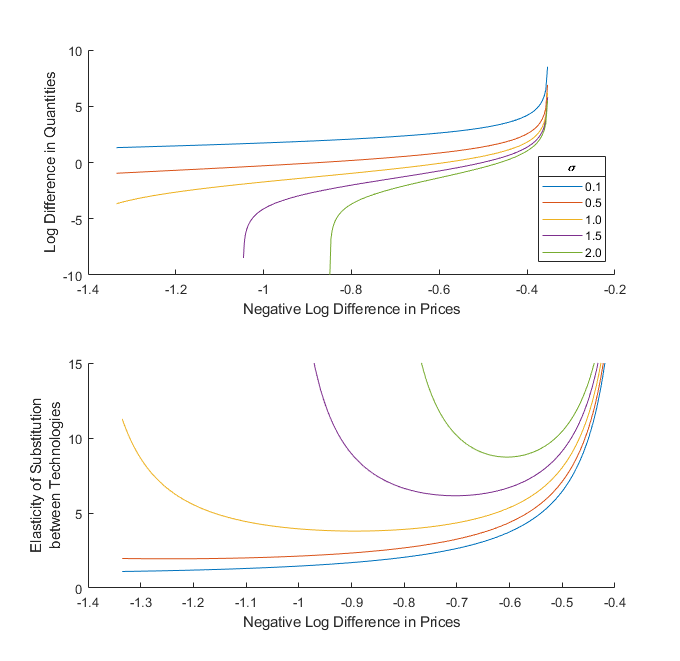
\includegraphics[width=1\linewidth]{../code/matlab/simulation_april/example_1_fig_1} \\
		\multicolumn{1}{@{\hspace{0.2in}}p{5.9in}@{}}{ \textit{Note: } The y-axis of the first plot is equivalent to $\log(X_1/X_2)$ and the x-axis of both plots is equivalent to  $\log(c_2/c_1)$. The legend in the upper subplot also applies to the lower subplot. These results were obtained using the following parameters: $\alpha_t = 0.6$, $\alpha_s = 0.4$, $\xi_1 = (1, \, 1)$, $\xi_2 = (1, \, 0.1)$, $c_1 = 104.3$, $c_2 = 60$. We plot results for various values of the intertemporal elasticity of substition for electricity consumption $\sigma$, which is used in the consumer's CES utility function. In order to numerically estimate these relationships, we first found the optimal quantities of $X$ over a range of prices $c_1^* \in (0.5\, c_1, 2 \,c_1)$. Then, we obtained estimates of the elasticity of substition by numerically differentiating $\log(X_1/X_2)$ with respect to $-log(c_1, c_2)$. That is, the elasticity of substitution between technology 1 and 2 is given by the slope of the upper subplot, and it is graphed in the lower subplot.   }     \\  
	\end{tabular}
\end{table}

We plot our numerical estimates of the elasticity of substitution between solar and coal power in \hyperref[fig:eosnum]{Figure 1}. These results were generated by computing the optimal quantities of each technology given a range of prices. Specifically, we held the price of solar constant and varied the price of coal from 50\% to 200\% of its original parametrized price. Then, we numerical differentiated $\log(X_1/X_2)$ with respect to $\log(c_2/c_1)$ to estimate the elasticity of substitution between solar and coal. This numerically computed elasticity of substitution $e$ on the production side is shown in the lower subplot. We repeat this process with different values of $\sigma$, the elasticity of substitution in the consumer's utility function. Recall that $\sigma < 1$ implies that  electricity consumption in different periods are complements, $\sigma = 1$ implies to a Cobb-Douglas relationship, and $\sigma > 1$ implies that electricity consumption in different periods are substitutes. Our results strongly suggest that a CES production structure does not accurately model intermittency. 

Firstly, note that the elasticity of substitution becomes increasingly non-linear as $\sigma$ rises. This is somewhat intuitive; when energy consumption can be substituted across periods, the market is more sensitive to the cost efficiency of technologies and less sensitive to when they produce. For instance, suppose we had two technologies that each produced in a different period; if consumers are less willing to substitute consumption across periods, both technologies are likely to be  employed, On the other hand, when consumers are open to substitution (implying large $\sigma$), they will simply consume the majority of their electricity in whichever period it is most cost effective to do so. Consequently, price plays bigger role than intermittency as $\sigma$ rises. This is further evident in the lower subplots; note that the numerical estimates of  $e$ rise as $\sigma$ rises. When consumers are less concerned about when they receive their energy, they are far more open to substituting between coal and solar power. 

Second, we find that $e$ approaches a "U" shape as $\sigma$ rises.... 

...Like \cite{HH} we find an S-shaped adoption curve for renewable energy driven by intermittency.\footnote{\citet{HH} reference \citet{Geroski2000} who provides a survey of the literature on adoption of new technologies. He finds that S-shaped adoption curves are often generated by information cascades. On the other hand, our model and that of Helm and Mier find S-shaped curves as a result of intermittency slowing down adoption.} 

\subsubsection{Externalities}


Often times, a social planner may also be interested in using other policy instruments such as research subsidies. In fact, \citet{Ace2012} find that both carbon taxes and research subsidies are necessary to promote long-run structural change in the energy production sector and avert a climate disaster. While our model focuses on production on a shorter time scale, we find a similar result -- a combination of both taxes and subsidies may be more effective in promoting a shift towards clean energy. 


Firstly, consider a case where a carbon tax is our only policy instrument. Additionally, suppose that our first technology produced negative externalities. Specifically, the social cost of pollution is given by $S(X) = \gamma X_1$ where $\gamma$ is the monetary damage per unit of $X_1$. A social planner is interested in balancing the damages caused by pollution with the surplus of the private sector and the revenue from the tax. That is, they aim to solve
$$\max_{\tau} \; CS + PS - S(X) + \tau X_1$$
where $\tau$ is the tax on $X_1$, so that its final price is $c_1 + \tau$ and the tax revenue is given by $\tau X_1$. The optimal tax is a Pigouvian tax; $\tau$ should be set equal to the marginal social cost of pollution $\gamma$. This is an expected, standard solution in most models.


%%% Pigouvian tax proof
\hfill \\
\begin{proof} We aim to maximize welfare with respect to the tax $\tau$, hence our first order condition is:
	\begin{align*}
	0 &= \frac{\partial CS}{\partial \tau} + \frac{\partial PS}{\partial \tau} - \frac{\partial S(X)}{\partial \tau} + \frac{\partial \tau X_1}{\partial \tau} \\
	&=  \left( \underbrace{\frac{\partial CS}{\partial p}  + \frac{\partial PS}{\partial p}}_{= 0} - \frac{ \partial  S(X)}{\partial p} + \frac{\partial \tau X_1}{\partial p} \right) \frac{\partial p}{\partial \tau} \\
	&=  - \gamma \frac{\partial  X_1}{\partial p} + \tau \frac{\partial  X_1}{\partial p}
	\end{align*}
	where the derivatives of producer and consumer surplus are eliminated by the envelope theorem. Therefore, we must have $\tau = \gamma$. \\
	\hfill
\end{proof}

Now, suppose that we may also subsidize research which improves the output efficiency of a technology. In particular, we let the output efficiency of technology 2 be $(\xi_{2t}, \, \xi_{2s})(1 + \beta)$ where $\beta$ is the percent improvement created by research. And, we let the cost of research be given by a convex, differentiable function $G(\beta)$. 


\hfill \\
\begin{proof} First, note that we have:
	$$X_1 = \dfrac{\alpha _{t}\,(1+\beta) \, \xi_{\mathrm{2s}}}{(c_{1}+ \tau)\,(1+\beta)\,\xi _{\mathrm{2s}}-c_{2}\,\xi _{\mathrm{1s}}}+\dfrac{\alpha _{s}\,(1+\beta)\,\xi _{\mathrm{2t}}}{(c_{1}+ \tau)\,(1+\beta)\,\,\xi _{\mathrm{2t}}-c_{2}\,\xi _{\mathrm{1t}}}$$		
	
	We aim to maximize welfare with respect to the tax $\tau$ and the research efficiency modifier $\beta$, hence our first order condition is:
	\begin{align*}
	0 	 &= \frac{\partial CS}{\partial \tau} + \frac{\partial PS}{\partial \tau} - \frac{\partial S(X)}{\partial \tau} + \frac{\partial \tau X_1}{\partial \tau}  - \frac{\partial G(\beta)}{\partial \beta}\\
	&=  \left( \underbrace{\frac{\partial CS}{\partial p}  + \frac{\partial PS}{\partial p}}_{= 0} - \frac{ \partial  S(X)}{\partial p} + \frac{\partial \tau X_1}{\partial p} - \frac{\partial G(\beta)}{\partial p} \right) \frac{\partial p}{\partial \tau} \\
	&=  - \gamma \frac{\partial  X_1}{\partial p} + \tau \frac{\partial  X_1}{\partial p} - \frac{\partial G(\beta)}{\partial p} \\
	\tau &= \gamma + \frac{\partial G(\beta)}{\partial X_1}
	\end{align*}
	where the derivatives of producer and consumer surplus are eliminated by the envelope theorem. Equivalently, if we take the derivative of the welfare function with respect to $\beta$, we find that:
	$$G(\beta) = -\gamma + \frac{\partial \tau}{\partial X_1}$$
	\hfill
\end{proof}

\pagebreak



\section{Empirical Methodology}

We aim to empirically estimate the intertemporal elasticity of substition for electricity consumption $\sigma$........

Recall our original first order condition (Equation 3) in the general model:
\begin{align*}
Z_t &= \left(\frac{\alpha_t}{p_t} \right)^\sigma \frac{I}{P} \\
P &= \sum_t \alpha_t^\sigma p_t^{1-\sigma}
\end{align*}
For any pair of electricity ouputs $Z_t$ and $Z_s$, we have:
$$\frac{Z_t}{Z_s} = \left(\frac{\alpha_t \, p_s}{\alpha_s \, p_t} \right)^\sigma \\$$
Taking logs on both sides and letting $i$ represent different observations, we may rewrite this in a form more suitable for estimation. 
\begin{align*}
\ln (Z_{t, i} / Z_{ s, i}) &= -\sigma \ln (P_{t,i} / P_{s,i}) + \sigma \ln (\alpha_{t,i} / \alpha_{s,i}) 
\end{align*}
Our data differentiates consumption for each state in the US, so we let $i$ refer to a particular state. Additionally, most consumers pay monthly fixed rates for electricity, so we can, at most, estimate this equation on a monthly basis; hence, $t$ and $s$ refer to different months. Lastly, note that the state $i$ is kept constant for each observation; this is because consumers within each state can substitute consumption across time, but consumers in different states do not substitute consumption with one another. 

In order to estimate this $\sigma$, we further modify the previous equation. 
Firstly, note that we cannot observe the demand shifter $\alpha_{t,i}$ directly, so we must replace the $\alpha$ terms with a set of controls that may be responsible for shifts in demand. So, still in general terms, our regression equation is now
\begin{align*}
\ln (Z_{t, i} / Z_{ s, i}) &= -\sigma \ln (P_{t,i} / P_{s,i}) +  \gamma_{t,i} A_{t,i} + \gamma_{s,i} A_{s,i} + u_i
\end{align*}
where $A$ represents set of controls for changes in demand while $u_i$ is a normal error term. Note that the control  $A_{t,i}$ replaces $\sigma \ln(\alpha_{t,i})$ and likewise for the period $s$ term; this substitution is valid because the $\ln(\alpha_{t,i}) \in \mathbb{R}$ and the $\sigma$ is simply absorbed into the estimated coefficient for $\gamma_{t,i}$. For the demand controls themselves, we choose to use heating (HDD) and cooling degree days (CDD) due to the aggregation of the data. That is, a more general control such as average temperature would not be able to directly capture intramonthly changes in demand, since variation in temperature would be lost when aggregated; on the other hand, CDDs and HDDs directly represent daily deviations in temperature even when totaled for each month. Additionally, demand for electricity may rise over time. Hence, we include, as a control, the difference in months between time $t$ and $s$; this is represented by $\Delta_{t,s}$. Finally, this panel requires us to consider fixed effects for each state, so we use a fixed effects panel regression. In total, the demand equation is:
\begin{align*}
\ln (Z_{ t, i} / Z_{ s, i}) &= -\sigma \ln (P_{t,i} / P_{s,i}) +  \gamma_{t,i} A_{t,i} + \gamma_{s,i} A_{s,i} + \eta \Delta_{t,s} + u_i \\
&= -\sigma \ln (P_{t,i} / P_{s,i}) +  \gamma_{t,i} \left( CDD_{t,i} + HDD{t,i} \right) \\
&\qquad + \gamma_{s,i} \left( CDD_{s,i} + HDD{s,i} \right)  + \eta \Delta_{t,s} + u_i
\end{align*}

Still, this equation may suffer from bias, since producers can also substitute production over time. For instance, it is possible to store fuel for electricity generation in the future when prices may rise. So, we define the following supply equation
\begin{align*}
\ln (Z_{ t, i} / Z_{ s, i}) &= \beta \ln (P_{t,i} / P_{s,i}) + \xi \ln (C_{t,i} / C_{s,i}) + v_{i}
\end{align*}
where $C_{t,i}$ is the average cost of coal used for electricity generation in state $i$ at time $t$ and $v_i$ is a normal error term. Coal prices are independent of the electricity demand error term $u_i$, since residential consumers do not generally use coal for electricity generation; on the other hand, shocks in the price of coal are linked with the supply of electricity. Hence, coal price is a theoretically valid instrument.  In total, the reduced form equation is given by:
$$ \ln (P_{t,i} / P_{s,i}) = \left( \beta + \sigma \right)^{-1} \left( \gamma_{t,i} A_{t,i} + \gamma_{s,i} A_{s,i} + \eta \Delta_{t,s} - \xi \ln (C_{t,i} / C_{s,i}) + u_{i} - v_i \right)  $$
where $A_{t,i}$ consists of CDDs and HDDs at time $t$. 

Finally, we also consider a semiparametric specification. That is, we allow the error terms $u_i$ and $v_i$ to be non-normal and place the demand controls and instruments in unknown functions. So, overall, we have:
\begin{align*}
\ln (Z_{ t, i} / Z_{ s, i}) &= -\sigma \ln (P_{t,i} / P_{s,i}) +  f \left( A_{t,i}, A_{s,i}, \Delta_{t,s} \right) + u_i \\
\ln (Z_{ t, i} / Z_{ s, i}) &= \beta \ln (P_{t,i} / P_{s,i}) + g \left( \ln (C_{t,i} / C_{s,i})  \right) + v_{i}
\end{align*}
where $f$ and $g$ are unknown, bounded functions. We restrict $cov(u_i, v_i) = 0$ but allow for the controls and instruments to be correlated. The advantage of this specification is that we can account for the controls or instrument having any nonlinear effects on the regressands. \textbf{(More here on explaining the estimation)}

\section{Data}

We collect monthly data from the EIA on retail electricity prices and consumption for each state in the US from 2011 to 2018. Additionally, also from the EIA, we collect monthly data on the average cost of coal for electricity generation. The coal price data set contains a large number of missing values due to privacy reasons; however, we do not expect that these missing values are correlated with the data itself. Finally, we collect data on HDDs and CDDs from the NCEP for the same panel. Then, we merge these three data sets and trim 1\% of outliers for a total of $826$ observations. We use this preliminary data set to construct the data required for our regressions. That is, each observation in our estimation equation belongs to a set $(t,s,i)$ consisting of two time periods and a state. Hence, we construct each row in our regression data set using unique combinations of $t,s$ where $t \neq s$ for each state $i$. Due to the number of potential combinations and thus observations, we restrict our data set to a random sample of 9000 observations.\footnote{We reran our regressions with several different samples of 9000 and found that our estimated coefficients did not significantly change; hence we believe this sample size is sufficient.}

\section{Results}

Based on the OLS results reported in \hyperref[table:1]{Table 1}, we estimate the intertemporal elasticity of substitution for electricity consumption $\hat{\sigma}  = 0.609$ ($|t| > 24$) when accounting for all degree day covariates and state fixed effects. Interestingly, we find that the estimated coefficients for all three specifications do not differ when considering fixed effects. Additionally, as expected, the coefficients on the degree day covariates are symmetrical; that is, the coefficient on $CDD_{t}$ is approximately the same as the negative of that on $CDD_{s}$, and the same applies to $HDD_{t}$ and $HDD_{s}$. On the other hand, we found that electricity consumption seems to rise more in response to CDDs rather than HDDs. Lastly, we find that the sign on $\Delta_{t,s}$ is positive in all regressions; this implies that electricity consumption rises over time independent of price. 

To account for endogeneity in the OLS results, we provide results for our IV specification in \hyperref[table:2]{Table 2}. Here, we find a much larger estimate $\hat{\sigma}  = 11.430$ ($|t| > 2.1$) when considering all covariates and fixed effects. F-Statistics on all three specifications are significantly larger than 10, which suggests that the instruments are not weak \citep{SS1997}. With respect to the demand controls, we find results similar to those of OLS. State fixed effects do not appear to affect the estimates, demand increases over time, and CDDs raise electricity consumption more than HDDs. 

Finally, we control for nonlinear effects using a partially linear IV regression reported in \hyperref[table:3]{Table 3}. Here, we find results similar to that of OLS; $\hat{\sigma} = 0.413$ ($|t| > 48$) when considering all controls. The estimate of $\sigma$ without any controls is not significantly different from that in specifications with controls. However, all of these estimates are significantly different from the IV results; hence, the IV regressions do not appear to be robust. Consequently, we opt to use these estimates of $\sigma$ in our model. Since these estimates show $\hat{\sigma} \in (0,1)$, it appears that electricity consumption in different months complement one another. 

\begin{table}[!htbp] \centering 
	\caption{OLS Regression Results}
	\label{table:1} 
	\small
	\begin{tabular}{@{\extracolsep{5pt}}lcccccc} 
		\\[-4ex]\hline  
		\hline \\[-1.8ex] 
		& \multicolumn{6}{c}{\textit{Dependent variable:} $\ln (Z_{ t, i} / Z_{ s, i})$} \\ [0.5ex]
		\cline{2-7} 
		\\[-1.8ex] & (1) & (2) & (3) & (4) & (5) & (6)\\ [0.5ex]
		\hline \\[-1.8ex] 
		$-\ln (P_{t,i} / P_{s,i})$ & 0.751$^{***}$ & 0.481$^{***}$ & 0.607$^{***}$ & 0.750$^{***}$ & 0.481$^{**}$ & 0.607$^{***}$ \\ 
		& (0.030) & (0.026) & (0.026) & (0.224) & (0.172) & (0.169) \\ 
		& & & & & & \\ 
		$\Delta_{t,s}$ &  &  & 0.001$^{***}$ &  &  & 0.001$^{***}$ \\ 
		&  &  & (0.0001) &  &  & (0.0002) \\ 
		& & & & & & \\ 
		CDD$_t$ &  & 0.990$^{***}$ & 1.003$^{***}$ &  & 0.990$^{***}$ & 1.002$^{***}$ \\ 
		$\quad(\times 1000^{-1})$&  & (0.016) & (0.016) &  & (0.087) & (0.086) \\ 
		& & & & & & \\ 
		CDD$_s$ &  & $-$0.999$^{***}$ & $-$1.011$^{***}$ &  & $-$0.999$^{***}$ & $-$1.012$^{***}$ \\ 
		$\quad(\times 1000^{-1})$&  & (0.016) & (0.016) &  & (0.087) & (0.085) \\ 
		& & & & & & \\ 
		HDD$_t$ &  & 0.306$^{***}$ & 0.294$^{***}$ &  & 0.307$^{***}$ & 0.295$^{***}$ \\ 
		$\quad(\times 1000^{-1})$&  & (0.005) & (0.005) &  & (0.030) & (0.030) \\ 
		& & & & & & \\ 
		HDD$_s$ &  & $-$0.309$^{***}$ & $-$0.296$^{***}$ &  & $-$0.308$^{***}$ & $-$0.295$^{***}$ \\ 
		$\quad(\times 1000^{-1})$&  & (0.005) & (0.005) &  & (0.029) & (0.029) \\ 
		& & & & & & \\ 
		Intercept & 0.001 & 0.002 & 0.002 &  &  &  \\ 
		& (0.003) & (0.006) & (0.006) &  &  &  \\ 
		& & & & & & \\  [0.9ex]
		\hline \\[-1.8ex] 
		State FEs &   &   &   & Yes & Yes & Yes \\ 
		Observations & 9,000 & 9,000 & 9,000 & 9,000 & 9,000 & 9,000 \\ 
		R$^{2}$ & 0.070 & 0.580 & 0.596 & 0.070 & 0.580 & 0.596 \\ 
		Adjusted R$^{2}$ & 0.070 & 0.579 & 0.596 & 0.065 & 0.577 & 0.594 \\ [0.5ex]
		\hline 
		\hline \\[-1.8ex] 
		\multicolumn{7}{@{}p{40em}@{}}{\textit{Note: } The sample covers all 50 US states from 2011 to 2018; outliers are removed by trimming 1\% of each variable except $\Delta_{t,s}$. The unit of observation is a set $(t,s,i)$ where $t \neq s$ are months and $i$ is a state; as discussed in the Data section, we take a random sample of 9000 observations from the data. The coefficient on $\ln (P_{t,i} / P_{s,i})$ is an estimate of $-\sigma$. The variable $\Delta_{t,s}$ is the difference in months between periods $t$ and $s$. CDD$_t$ and HDD$_t$ refer to the total number of heating and cooling degree days in month $t$. Robust standard errors are reported in parentheses. *p$\textless$0.05, **p$\textless$0.01, ***p$\textless$0.001}  \\ 
	\end{tabular} 
\end{table}





\begin{table}[!htbp] \centering 
	\caption{IV (2SLS) Regression Results}
	\label{table:2} 
	\small
	\begin{tabular}{@{\extracolsep{4pt}}lcccccc} 
		\\[-4ex]\hline  
		\hline \\[-1.6ex] 
		& \multicolumn{3}{c}{First-Stage} & \multicolumn{3}{c}{Second-Stage} \\ [0.5ex]
		& \multicolumn{3}{c}{\textit{Dep. Variable:} $\ln (P_{t,i} / P_{s,i})$ } & \multicolumn{3}{c}{\textit{Dep. Variable:}  $\ln (Z_{ t, i} / Z_{ s, i})$}\\ [0.5ex]
		\cmidrule(lr){2-4} \cmidrule(lr){5-7}\\[-2.2ex] 
		& (A.1) & (B.1) & (C.1) & (A.2) & (B.2) & (C.2)\\ [0.5ex]
		\hline \\[-1.8ex] 
		$ \ln (C_{t,i} / C_{s,i})$ & $-$0.060$^{***}$ & 0.004$^{*}$ & 0.004$^{*}$ &  &  &  \\ 
		& (0.002) & (0.002) & (0.002) &  &  &  \\ 
		& & & & & & \\ 
		$-\ln (P_{t,i} / P_{s,i})$ &  &  &  & 0.711$^{***}$ & 13.987 & 11.430$^{*}$ \\ 
		&  &  &  & (0.106) & (8.384) & (5.330) \\ 
		& & & & & & \\ 
		$\Delta_{t,s}$  &  & 0.001$^{***}$ & 0.001$^{***}$ &  &  & 0.007$^{*}$ \\ 
		&  & (0.00002) & (0.00002) &  &  & (0.003) \\ 
		& & & & & & \\ 
		CDD$_t$  &  & 0.151$^{***}$ & 0.151$^{***}$ &  & 3.064$^{*}$ & 2.620$^{**}$ \\ 
		$\quad(\times 1000^{-1})$&  & (0.007) & (0.007) &  & (1.288) & (0.798) \\ 
		& & & & & & \\ 
		CDD$_s$  &  & $-$0.149$^{***}$ & $-$0.149$^{***}$ &  & $-$3.034$^{*}$ & $-$2.609$^{***}$ \\ 
		$\quad(\times 1000^{-1})$&  & (0.007) & (0.007) &  & (1.264) & (0.788) \\ 
		& & & & & & \\ 
		HDD$_t$  &  & $-$0.057$^{***}$ & $-$0.057$^{***}$ &  & $-$0.407 & $-$0.311 \\ 
		$\quad(\times 1000^{-1})$&  & (0.003) & (0.003) &  & (0.447) & (0.301) \\ 
		& & & & & & \\ 
		HDD$_s$  &  & 0.058$^{***}$ & 0.058$^{***}$ &  & 0.423 & 0.324 \\ 
		$\quad(\times 1000^{-1})$&  & (0.003) & (0.003) &  & (0.458) & (0.308) \\ [0.9ex]
		\hline \\[-1.8ex] 
		State FEs &  Yes & Yes  & Yes  & Yes & Yes & Yes \\ 
		Observations & 9,000 & 9,000 & 9,000 & 9,000 & 9,000 & 9,000 \\ 
		R$^{2}$          & 0.066 & 0.441 & 0.441 & & &  \\ 
		Adjusted R$^{2}$ & 0.066 & 0.441 & 0.441 & & &  \\ 
		F Statistic & 678$^{***}$ & 1,213$^{***}$ & 1,197$^{***}$  &  &  &  \\ 
		\hline 
		\hline \\[-1.8ex] 
		\multicolumn{7}{@{}p{39.2em}@{}}{\textit{Note: } The log difference in coal price between period $t$ and $s$, $ \ln (C_{t,i} / C_{s,i})$, is used as an instrument in these regressions. The sample covers all 50 US states from 2011 to 2018; outliers are removed by trimming 1\% of each variable except $\Delta_{t,s}$. The unit of observation is a set $(t,s,i)$ where $t \neq s$ are months and $i$ is a state; as discussed in the Data section, we take a random sample of 9000 observations from the data. The coefficient on $\ln (P_{t,i} / P_{s,i})$ is an estimate of $-\sigma$. The variable $\Delta_{t,s}$ is the difference in months between periods $t$ and $s$. CDD$_t$ and HDD$_t$ refer to the total number of heating and cooling degree days in month $t$. Robust standard errors are reported in parentheses. *p$\textless$0.05, **p$\textless$0.01, ***p$\textless$0.001}  \\ 
	\end{tabular} 
\end{table}


\begin{table}[!htbp] \centering 
	\caption{Partially Linear IV Regression Results}
	\label{table:3} 
	\small
	\begin{tabular}{@{\extracolsep{4em}}lccc} 
		\\[-4ex]\hline  
		\hline \\[-1.8ex] 
		& \multicolumn{3}{c}{\textit{Instrument: $ \ln (C_{t,i} / C_{s,i})$}} \\ 
		\cline{2-4} 
		%\\[-1.8ex] & ln\_load\_rel \textasciitilde ln\_price\_rel & ln\_load\_rel \textasciitilde (CDD\_1) & ln\_load\_rel \textasciitilde time\_diff + (CDD\_1) \\ 
		\\[-1.8ex] & (1) & (2) & (3)\\ [0.5ex]
		\hline \\[-1.8ex] 
		$\hat{\sigma} $ & 0.5676$^{***}$ & 0.4511$^{***}$ & 0.4129$^{***}$ \\ 
		& (0.1036) & (0.0042) & (0.0085) \\ [0.9ex]
		\hline \\[-1.8ex] 
		Time Control &   &   & Yes  \\ 
		Degree Day Controls &   & Yes  & Yes  \\ 
		Observations & 9,000 & 9,000 & 9,000 \\
		\hline 
		\hline \\[-1.8ex] 
		\multicolumn{4}{@{}p{36em}@{}}{\textit{Note: } The log difference in coal price between period $t$ and $s$, $ \ln (C_{t,i} / C_{s,i})$, is used as an instrument in these regressions. The sample covers all 50 US states from 2011 to 2018; outliers are removed by trimming 1\% of each variable except $\Delta_{t,s}$. The unit of observation is a set $(t,s,i)$ where $t \neq s$ are months and $i$ is a state; as discussed in the Data section, we take a random sample of 9000 observations from the data. The estimation procedure is described in the appendix.  Robust standard errors are reported in parentheses. *p$\textless$0.05, **p$\textless$0.01, ***p$\textless$0.001}  \\ 
	\end{tabular} 
\end{table} 

\pagebreak

\section{Conclusion}

An aim for future research may be to develop a model of clean and dirty energy that incorporates both predictable and stochastic intermittency in a multi-period setting. 



\pagebreak



\section{Literature}

\begin{itemize}
	\item \cite{Delarue} develop a model that distinguishes between power and energy in order to split up costs and risks into fixed and variable factors. 
	\item \cite{SB2018} look at interactions between different solar and wind installations (covar matrix), while many other energy models do not.
\end{itemize}


\begin{thebibliography}{9}
	
	\bibitem[Acemoglu et al.(2012)]{Ace2012}
	Acemoglu, D., Aghion, P., Bursztyn, L., \& Hemous, D. (2012). The Environment and Directed Technical Change. American Economic Review, 102(1), 131–166. https://doi.org/10.1257/aer.102.1.131
	\bibitem[Ambec and Crampes (2012)]{AC2012}
	Ambec, S., \& Crampes, C. (2012). Electricity provision with intermittent sources of energy. Resource and Energy Economics, 34(3), 319–336. https://doi.org/10.1016/j.reseneeco.2012.01.001
	
	\bibitem[Borenstein(2012)]{Boren2012}
	Borenstein, S. (2012). The Private and Public Economics of Renewable Electricity Generation. Journal of Economic Perspectives, 26(1), 67–92. https://doi.org/10.1257/jep.26.1.67
	
	\bibitem[Chao(2011)]{Chao2011}
	Chao, H. (2011). Efficient pricing and investment in electricity markets with intermittent resources. Energy Policy, 39(7), 3945–3953. https://doi.org/10.1016/j.enpol.2011.01.010
	
	\bibitem[Delarue et al.(2010)]{Delarue}
	Delarue, E., De Jonghe, C., Belmans, R., \& D’Haeseleer, W. (2010). Applying portfolio theory to the electricity sector: Energy versus power. Energy Economics, 33(1), 12–23. https://doi.org/10.1016/j.eneco.2010.05.003
	
	\bibitem[EIA(2019a)]{EIANetgen}
	Electricity Information Administration (2019). Net generation, United States, all sectors, annual. Electricity Data Browser. https://www.eia.gov/electricity/data/browser
	
	\bibitem[EIA(2019b)]{EIALCOE}
	Electricity Information Administration (2019). Levelized Cost and Levelized Avoided Cost of New Generation. Annual Energy Outlook 2019. https://www.eia.gov/outlooks/aeo/pdf/electricity\_generation.pdf
	
	\bibitem[Foley et al.(2012)]{Foley2012}
	Foley, A., Leahy, P., Marvuglia, A., \& Mckeogh, E. (2012). Current methods and advances in forecasting of wind power generation. Renewable Energy, 37(1), 1–8. https://doi.org/10.1016/j.renene.2011.05.033
	
	\bibitem[Geroski(1957)]{Geroski2000}
	Geroski, P. (2000). Models of technology diffusion. Research Policy. Elsevier B.V. https://doi.org/10.1016/S0048-7333(99)00092-X
	
	\bibitem[Helm and Mier(2019)]{HH}
	Helm, C., \& Mier, M. (2019). On the efficient market diffusion of intermittent renewable energies. Energy Economics, 80, 812–830. https://doi.org/10.1016/j.eneco.2019.01.017
	
	\bibitem[Joskow(2011)]{Joskow2011}
	Joskow, P. (2011). Comparing the Costs of Intermittent and Dispatchable Electricity Generating Technologies. American Economic Review, 101(3), 238–241. https://doi.org/10.1257/aer.101.3.238
	
	\bibitem[Mohajeryami et al.(2016)]{Moha2016}
	Mohajeryami, S., Moghaddam, I., Doostan, M., Vatani, B., \& Schwarz, P. (2016). A novel economic model for price-based demand response. Electric Power Systems Research, 135, 1–9. https://doi.org/10.1016/j.epsr.2016.03.026
	
	\bibitem[Musgens and Neuhoff(2006)]{MN2006}
	Musgens, F., \& Neuhoff, K. (2006). Modelling Dynamic Constraints in Electricity Markets and the Costs of Uncertain Wind Output. Faculty of Economics.
	
	\bibitem[Neuhoff et al.(2007)]{NCK2007}
	Neuhoff, K., Cust, J. \& Keats, K. (2007). Implications of intermittency and transmission constraints for renewables deployment. Cambridge Working Papers in Economics 0711, Faculty of Economics, University of Cambridge.
	
	\bibitem[ORNL(2004)]{ORNL}
	ORNL (2004). Measurement practices for reliability and power quality. A toolkit of reliability measurement practices. U.S. Department of Energy. https://info.ornl.gov/sites/publications/Files/Pub57467.pdf
	
	\bibitem[Schwarz et al.(2002)]{Schwarz}
	Schwarz, P., Taylor, T., Birmingham, M., \& Dardan, S. (2002). INDUSTRIAL RESPONSE TO ELECTRICITY REAL‐TIME PRICES: SHORT RUN AND LONG RUN. Economic Inquiry, 40(4), 597–610. https://doi.org/10.1093/ei/40.4.597
	
	\bibitem[Shahriari and Blumsack(2018)]{SB2018}
	Shahriari, M., \& Blumsack, S. (2018). The capacity value of optimal wind and solar portfolios. Energy, 148, 992–1005. https://doi.org/10.1016/j.energy.2017.12.121
	
	\bibitem[Staiger and Stock(1997)]{SS1997} 
	Staiger, D., \& Stock, J. (1997). Instrumental Variables Regression with Weak Instruments. Econometrica, 65(3), 557–586. https://doi.org/10.2307/2171753
	
	\bibitem[Warkins and Knight(1922)]{Knight}
	Watkins, G., \& Knight, F. (1922). Knight’s Risk, Uncertainty and Profit. The Quarterly Journal of Economics, 36(4), 682–690. https://doi.org/10.2307/1884757
	
	
	%		\bibitem[Angel, Harris, and Spatt(2011)]{Angel} 
	%		Angel, J.J., Harris, L.E., \& Spatt, C. S. (2011). Equity Trading in the 21st Century. Quarterly Journal Of Finance, 1(1), 1-53.
	
	%		\bibitem[Stern(2012)]{Stern} 
	%		Stern, D. (2012). “Interfuel Substitution: A Meta-Analysis.” Journal of Economic Surveys 26 (2): 307–331. \href{https://doi.org/10.1111/j.1467-6419.2010.00646.x}{https://doi.org/10.1111/j.1467-6419.2010.00646.x}.
	
	
	
\end{thebibliography}	
	
\end{document}





